\documentclass{article}[a4paper,12pt]
\usepackage[utf8]{inputenc}
\usepackage{amsmath,amssymb,amsthm,amsfonts,mathtools}
\usepackage[inline]{enumitem}
\usepackage{soul}
\usepackage{cancel}
\usepackage{hyperref}
\usepackage{centernot}
\usepackage{pifont}
\usepackage{changepage}
\usepackage{subcaption}
\usepackage[section]{placeins}
\usepackage{lipsum, graphicx, caption}
\usepackage{array}
\usepackage{float}
\usepackage{commath}
\usepackage{wrapfig}
\usepackage{amsmath}
\usepackage{amsfonts}
\usepackage{amssymb}
\theoremstyle{definition}
\newtheorem{innercustomgeneric}{\customgenericname}
\providecommand{\customgenericname}{}
\newcommand{\newcustomtheorem}[2]{%
  \newenvironment{#1}[1]
  {%
   \renewcommand\customgenericname{#2}%
   \renewcommand\theinnercustomgeneric{##1}%
   \innercustomgeneric
  }
  {\endinnercustomgeneric}
}
\newcustomtheorem{customthm}{Theorem}
\newcustomtheorem{customlem}{Lemma}
\newcustomtheorem{customdefn}{Definition}
\newcustomtheorem{customprop}{Proposition}
\newcustomtheorem{customexer}{Exercise}
\renewcommand{\qedsymbol}{$\blacksquare$}

\setlength\parindent{0pt}
\let\emptyset\varnothing
\usepackage{geometry}
\geometry{
	a4paper, portrait,
	total = {170mm,257mm},
	left = 20mm,
	top = 20mm,
}

\usepackage{xcolor}
\usepackage{pagecolor}
\pagecolor{white}
\color{black}

\title{\textbf{AI For Everyone}}
\author{
	\textbf{Om Prabhu}\\
	19D170018\\
	Undergraduate, Department of Energy Science and Engineering\\
	Indian Institute of Technology Bombay\\}
\date{Last updated \today}

\begin{document}
\maketitle
\vspace{-12pt}
\hrulefill
\vspace{6pt}

\textbf{NOTE:} This document is a brief compilation of my notes taken during the `AI For Everyone' course by \texttt{\href{https://www.deeplearning.ai/}{deeplearning.ai}}. You are free to read and modify it for personal use. You may check out the course here: \texttt{\href{https://www.coursera.org/learn/ai-for-everyone}{https://www.coursera.org/learn/ai-for-everyone}}.

\hrulefill
\tableofcontents
\vspace{6pt}

\hrulefill
\pagebreak

\section{Introduction}
\subsection{About myself}
Hello. I am Om Prabhu, currently an undergrad at the Department of Energy Science and Engineering, IIT Bombay. If you have gone through my website (\texttt{\href{https://omprabhu31.github.io/}{https://omprabhu31.github.io/}}) earlier, which is probably where you found this document too, you will know that I am quite a bit into programming and tinkering with code to try and do cool stuff. Additionally, I love playing video games, listening to music and engaging in a little bit of creative writing as and when I get time. With this brief self-introduction, let us get into why I decided to pursue this course.
\subsection{About this course}
As you probably know, AI (artificial intelligence) is rapidly changing the way we work and live. It is difficult to name industries which are not likely to be impacted by AI in the near future (I initially thought of the textile industry as an example, but a simple Google search proved exactly how wrong I was). AI is generating huge amounts of industrial revenue per year and is likely to create 13 trillion US dollars per year by the time we reach 2030 (source: McKinsey Global Institute).
\vspace{6pt}

Hence, it is important to gain at least a general overview of the what makes AI such a powerful tool. Right off the bat, one of the major reasons why AI has taken off recently is due to the rise of neural networks and deep learning. But this is not all. One needs to learn what types of data are valuable to AI and how the type and amount of data influences the performance of a neural network. Further, it is also important to know how AI can be used to build personal as well as company projects. Lastly, it is also important to know how AI will affect society and jobs so that one is better able to understand AI technology and navigate this rise of AI.
\vspace{6pt}

With all this said, let us try to understand what AI really is and accomplish the above objectives.

\hrulefill
\pagebreak
\section{What is AI?}
AI is a very happening industry today and there is a lot of excitement among people as to how the rise of AI will map out. While this has boosted development of AI technologies even further, it has also lead to irrational fears among society. One of the major reasons for this is because not many people realize that AI can actually be put into 2 separate categories:
\begin{itemize}
	\item ANI (artificial narrow intelligence): can do one thing (eg: smart speaker, self driving car, web search algorithms); incredibly valuable in specific industries due to narrow application
	\item AGI (artificial global intelligence): can do anything a human can do (perhaps even more things)
\end{itemize}
While the world has seen tremendous progress with ANIs, the same cannot be said for AGIs. This lack of distinction between ANIs and AGIs is what has led to fears of super-intelligent robots taking over the world.
\vspace{6pt}

In this section, we will be mainly looking at what ANIs can do and how to apply them to real-world problems.
\subsection{Machine Learning}
The rise of AI has been driven by one major tool known as Machine Learning. While the term might give a characteristic of omniscience to machines, this is far from true. In fact, the most used form of ML is what is known as Supervised Learning (or A $\rightarrow$ B mapping):
\begin{itemize}
	\item learning a function that maps input to output based on a database of example I/O pairs
	\item learning algorithm analyses example training data to generate a function to map new examples
	\item eventually the algorithm can \textit{learn} to predict the target output in previously unseen situations
\end{itemize}
One major application of this technology is in the online advertising industry. The input is in the form of advertisement details \& some user info based on which the AI algorithm tries to figure out if the user will click on the ad or not. This is how users are shown only a certain set of advertisements online.
\vspace{6pt}

Another application of supervised learning lies in self driving cars. The input is a set of images \& some radar info from sensors on the car. The AI uses this data to output the position of nearby cars and/or obstacles so that the self-driving car can avoid them. 
\vspace{6pt}

Surely the concept of merely taking the input to construct an output seems limiting in the general sense of the scope of AI, however it can evidently be very valuable once a suitable application scenario is found. Now while the idea of supervised learning has been around for decades, it has taken off only in the recent years. This is mainly because of the limitation of technology to train large sets of neural networks to process huge amounts of data while also improving AI performance. This can be illustrated through a graph as follows:
\begin{center}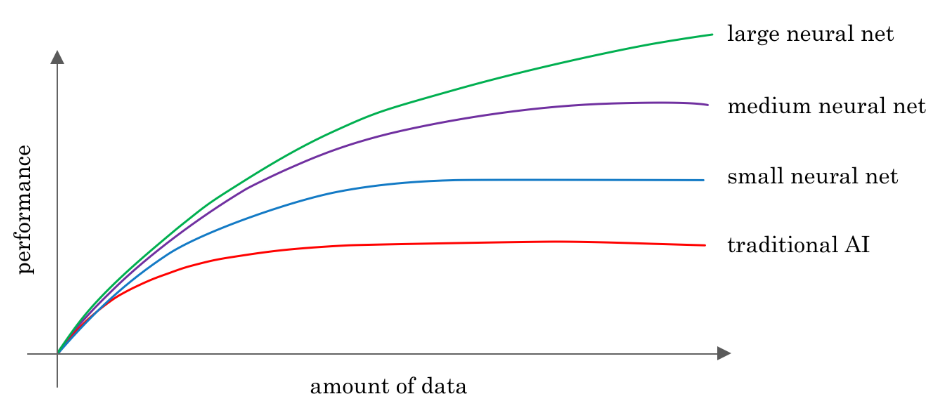
\includegraphics[width=\textwidth]{data_vs_performance.png}\end{center}
\begin{itemize}
	\item for traditional AI systems, the data vs performance graph maxes out pretty early
	\item on training increasingly complex neural networks with higher amounts of data, performance keeps on getting better for much longer  
\end{itemize}
Hence to achieve the highest performance levels, we need two things. Firstly, it helps to have a lot of data - this is where terms like `big data' come in. Additionally, we need the ability to train large sets of neural networks, which is made possible by specialized processors like advanced GPUs.
\subsection{Data}
Data is one of the 2 main things required to improve performance of AI systems. But simply having lots of data is not always helpful - we need to have the right type of data in the right format (structured or unstructured). Let's take a look at an example of a `dataset' (or a table of data):
\begin{center}
\begin{tabular}{|c|c|c|}
\hline
\textsc{Size of house (sqft)} & ... & \textsc{Price of house} (1000\$)\\
\hline
548 &  & 119\\
\hline
679 &  & 167\\
\hline
834 &  & 233\\
\hline
1209 &  & 342\\
\hline
1367 &  & 399\\
\hline
\end{tabular}
\end{center}
In practice, we will need a lot more than just 5 data entries to build an AI system, but let's work with this for now. The above dataset could work for an AI which checks whether houses are priced appropriately or not. In this case, the input would be the size of the house and the output would be the price. Going further, we might try to improve our AI by adding more input data fields such as the number of bedrooms, location, etc.
\vspace{6pt}

Another application of the same dataset would be figuring out the most appropriate house for a consumer on a fixed budget. In this case, our input and output fields will be exactly the opposite compared to the first application. What this means in essence is that, given a dataset, it is up to us to decide what is the input and what is the output, and how to choose these definitions to bring out the maximum value to our product.
\subsubsection{Collection of data}
So far, we have established that data is an important tool for AI systems and that there is a certain flexibility regarding the choice of input and output. But how do we get data? To discuss this, let us now switch to the more traditional example in machine learning of an algorithm designed to recognize images of cats:
\begin{itemize}
	\item manual labelling: collect a set of pictures and manually label them as `cat' or `not cat'
	\begin{itemize}
		\item[$-$] tried and true way of obtaining a highly reliable dataset having both input and output fields
		\item[$-$] difficult, given the huge amount of data required (usually on the scale of several thousands of entries)
	\end{itemize}
	\item observing behaviours
	\begin{itemize}
		\item[$-$] user behaviour: e-commerce websites keeping a tab on prices offered to users and whether they bought the product or not, something like this:
	\end{itemize}
\end{itemize}
\begin{center}
\begin{tabular}{|c|c|c|c|}
\hline
\textsc{User ID} & \textsc{Time} & \textsc{Price} (\$) & \textsc{Purchased}\\
\hline
0156 & Feb 22, 09:19:19 & 19.07 & No\\
\hline
1548 & Apr 01, 23:34:56 & 23.01 & Yes\\
\hline
4898 & May 23, 11:59:02 & 18.72 & Yes\\
\hline
8896 & Jul 10, 17:42:37 & 16.55 & No\\
\hline
\end{tabular}
\end{center}
\begin{itemize}
	\item[]
	\begin{itemize}
		\item[$-$] machine behaviour:  fault prediction in machines based on operating conditions, something like this:
	\end{itemize}
\end{itemize}
\begin{center}
\begin{tabular}{|c|c|c|c|}
\hline
\textsc{Machine ID} & \textsc{Temperature (K)} & \textsc{Pressure (atm)} & \textsc{Fault}\\
\hline
55132 & 332 & 10.96 & Yes\\
\hline
29475 & 378 & 8.22 & Yes\\
\hline
00826 & 489 & 5.78 & No\\
\hline
19475 & 653 & 2.99 & No\\
\hline
\end{tabular}
\end{center}
\begin{itemize}
	\item download from internet/partnerships: pre-compiled datasets that can be readily downloaded from the web (after obtaining required licenses if any), or obtained from partners (eg: a company obtaining fault analysis datasets from machine manufacturers)
\end{itemize}
\subsubsection{Misconceptions about data}
When thinking about the use of data, many people believe that they should have a lot of data on hand before feeding it into an AI system, and that having vast amounts of data will ensure the success of the AI system. Here's why this may not always work in practice:
\begin{itemize}
	\item more data does NOT mean a perfect dataset
	\begin{itemize}
		\item better to start relatively small and keep on continuously feeding data to the AI team
		\item more often than not, the AI team provides dynamic feedback to the IT team regarding what data is useful and what type of IT infrastructure to invest in
	\end{itemize}
	\item do NOT assume the success of an AI team just because it has a lot of data $-$ garbage in, garbage out
	\begin{itemize}
		\item not all data is valuable, `bad' data will lead to AI learning inaccurate things
		\item processing huge amounts of data needs appropriate infrastructure to complement it
	\end{itemize}
\end{itemize}
There are many more data problems that may arise in practice, like:
\begin{itemize}
	\item incorrect/missing values, or incomplete data: refer to the below example
\end{itemize}
\begin{center}
\begin{tabular}{|c|c|c|}
\hline
\textsc{Size of house (sqft)} & \textsc{No. of bedrooms} & \textsc{Price of house} (1000\$)\\
\hline
548 & 1 & 119\\
\hline
679 & 1 & 0.001\\
\hline
834 & 2 & unknown\\
\hline
unknown & 3 & 342\\
\hline
1367 & 54 & 399\\
\hline
\end{tabular}
\end{center}
\begin{itemize}
	\item multiple types of data: AI algorithms work very well for all types of data, but techniques for dealing with them might vary
	\begin{itemize}
		\item unstructured data: images, audio, video, text documents
		\item structured data: tables, spreadsheets, databases
	\end{itemize}
\end{itemize}
\subsection{AI terminology}
Up till now, we've been throwing around terms like AI, machine learning, neural networks, etc. Let's briefly explore what these terms actually mean.
\subsubsection{Machine learning vs. data science}
There is a thin line between what can be interpreted as machine learning and as data science. Let's say we have a dataset of houses like the one below:
\begin{center}
\begin{tabular}{|p{7em}|p{6em}|p{6em}|p{6em}|p{8em}|}
\hline
\textsc{Size of house (sqft)} & \textsc{No. of bedrooms} & \textsc{No. of bathrooms} & \textsc{Newly renovated} & \textsc{Price of house} (1000\$)\\
\hline
548 & 1 & 2 & N & 119\\
\hline
679 & 1 & 2 & N & 167\\
\hline
834 & 2 & 3 & Y & 233\\
\hline
1209 & 3 & 4 & Y & 342\\
\hline
1367 & 4 & 2 & N & 399\\
\hline
\end{tabular}
\end{center}
An application of this dataset to help construction companies price  houses appropriately with the first 4 columns as input and the price as output would be a machine learning system, and particularly a supervised learning system. ML often results in running AI systems used on a mass scale.
\vspace{6pt}

In contrast, another application of the dataset is to actually let a team analyse the data in order to gain insights. They might come up with certain conclusions based on this, for example `Houses with 3 bedrooms are pricier than 2 bedrooms of a similar size'. This can help companies take decisions on whether to build houses with 2 or 3 bedrooms, whether to renovate houses in order to sell them for a higher price, etc. This is an example of a data science project, where the output is a set of conclusions that helps companies take business decisions.
\vspace{6pt}

Let's take the online advertising industry as another example. Personalized ads powered by AI systems (that take ad info and user info as input and determine if the user will click on the ad or not) are machine learning systems. However when business teams analyse trends in the industry and come up with conclusions like `the textile industry is not buying a lot of ads, but could be convinced otherwise with the right sales approach', it becomes a part of data science.
\subsubsection{Deep learning}
Let's take the same example of pricing houses. We take the 4 columns on the left as input. One of the most effective ways of generating the output would be to feed it into what are called neural networks.
\begin{center}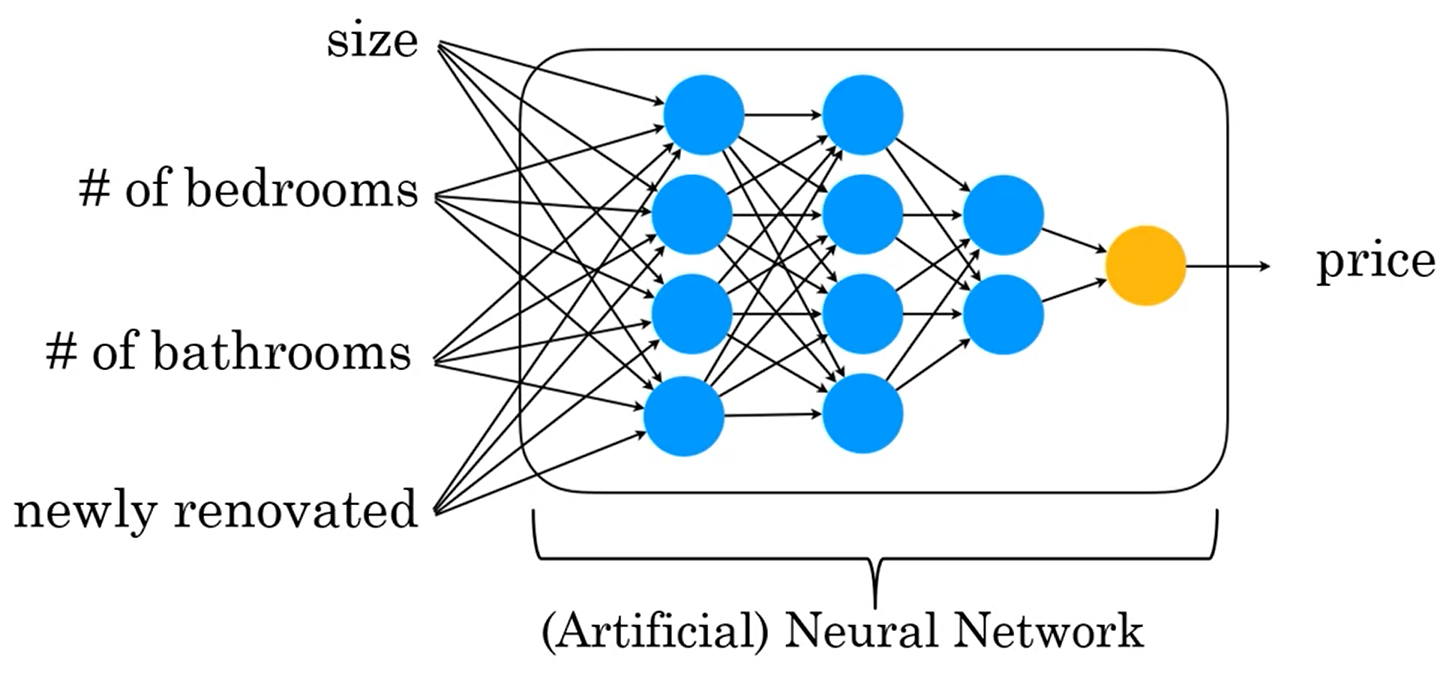
\includegraphics[width=\textwidth]{neural_network.png}\end{center}
These are pretty similar to the network of neurons spread across the human body (which is also why they are referred to as artificial neural nets). This representation of ANNs bears some resemblance to the brain in that the blue circles are called artificial neurons which relay information across the network. And the resemblance ends right here. The details of how ANNs work are completely unrelated to how the human brain works. 
\vspace{6pt}

At the end, what an ANN boils down to is nothing but a big mathematical equation that leads the system to reach the output based on a set of input parameters. This makes them very effective for learning A $\rightarrow$ B mappings. The terms `deep learning' and `neural networks' are used almost interchangeably today.
\subsubsection{The larger picture}
If we were to construct a Venn diagram showing all the concepts above, we would probably have something like this:
\begin{center}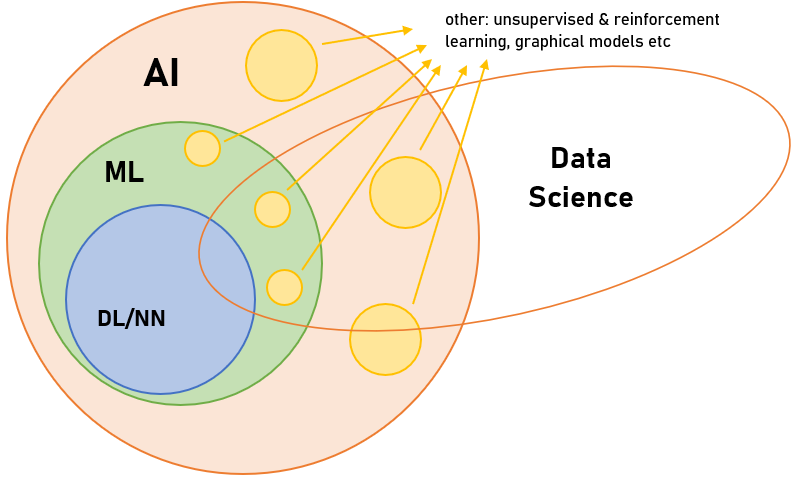
\includegraphics[scale=0.8]{ai_terminology.png}\end{center}
To date, there is a discrepancy about how data science fits into this picture. Some say AI is a subset of data science while others say the opposite. However, it is better seen as a cross-cutting subset that comprises of all these tools from AI and also other tools that drive business insights.
\subsection{AI companies}
In this era, it is possible for almost any company to employ a few deep learning algorithms. However, that by itself does not necessarily make it an AI company. AI companies specialize in the following:
\begin{itemize}
	\item strategic data acquisition: many AI companies have free products solely for the purpose of acquiring data that can be better monetized elsewhere
	\item unified data warehouses: pre-emptive investments in bringing data together to a unified warehouse/a small set of connected warehouses 
	\item pervasive automation: inserting AI algorithms to automate certain generic tasks in order to apply human labour \& intelligence in more specialised work roles
	\item specialized roles: such as machine learning engineers (MLEs); allows for better division of labour and assigning specialized tasks to increase efficiency
\end{itemize}
It turns out that there is a systematic process using which companies can implement many of the above strategies to ensure that they use AI to their maximum benefit:
\begin{enumerate}
	\item execute pilot projects to gain momentum and get a better sense of what AI can and cannot do, what types of data are useful, etc
	\item bring together an AI team and provide extensive AI training to engineers as well as managers \& executives
	\item develop an AI strategy and build IT infrastructure based on dynamic feedback from the AI team
	\item align internal and external communications so that others in the company hierarchy (shareholders, customers, etc) know how to navigate the rise of AI
\end{enumerate}
\subsection{Limitations of AI}
Before committing to an AI project, it is important to check whether it is feasible. While the success stories we read in articles might make it sound like AI knows no bounds, this is far from reality. There are several limitations (currently, at least) as to what AI can and cannot do.
\vspace{6pt}

As an imperfect rule of thumb, anything that a human can do within a few seconds of thought can probably be automated using AI - for example, telling whether a phone is scratched/dented, looking around and determining positions of cars, deciphering audio, etc. In constrast, an AI probably cannot write a 50-page report based on in-depth analysis of the stock market. Let us take a look at some more examples:
\begin{itemize}
	\item customer support automation: can sort incoming emails and redirect them to appropriate sections of customer support; cannot type out personalized responses
\end{itemize}
\begin{center}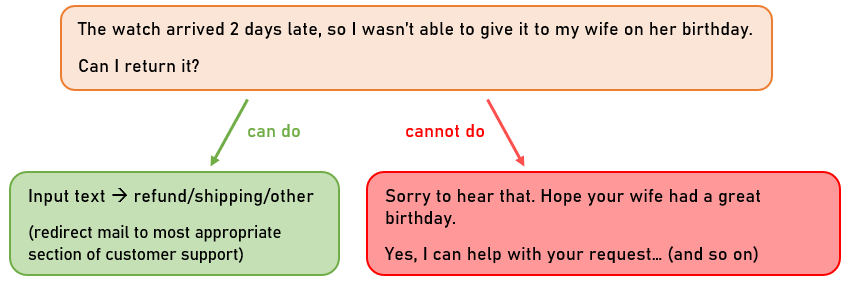
\includegraphics[width=\textwidth]{customer_support_automation.png}\end{center}
What if we try to do this anyway? Say we have a deep learning algorithm ready and a decent sized dataset of 1000 user emails and appropriate responses. We would get something like this:
\begin{center}
``My product is damaged." $\rightarrow$ ``Thank you for your email."

``Where can I write a review?" $\rightarrow$ ``Thank you for your email."

``How do I send a product as a gift?" $\rightarrow$ ``Thank you for your email."
\end{center}
It turns out that a sample size of 1000 (or even 100,000 as a matter of fact) is just not enough for an AI algorithm to write out appropriate and empathetic responses. In some cases, the AI may even generate gibberish which is clearly not desired.
\begin{itemize}
	\item self-driving car: can use sensors and photographs to figure out relative positions of other cars; cannot respond appropriately to human gestures
\end{itemize}
\begin{center}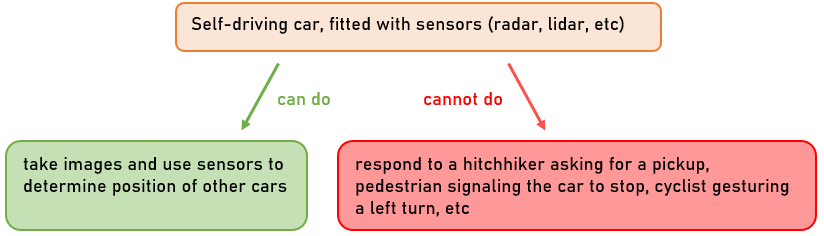
\includegraphics[width=\textwidth]{self_driving_car.png}\end{center}
One of the main reasons why this is so difficult to do is due to the sheer amount of possible hand gestures that could be made by humans. It is difficult to collect data of tens of thousands of people performing gestures. And again if we try to do it anyway, the consequences would be even harsher than in the scenario of customer support above.
\begin{itemize}
	\item X-ray diagnosis: can diagnose diseases from around 10,000 labelled images (difficult to collect for rare diseases); cannot diagnose diseases based on a small set of images in a medical textbook (a human doctor can do this, however)
\end{itemize}
In the context of X-ray diagnosis, we can make out another weakness of AI, that is when it is asked to work with new types of data. Let's say the sample data contains high quality X-ray images. The AI algorithm will most likely fail when faced with poor-quality X-ray scans or images from even a slightly defective machine.
\vspace{6pt}

In the end, there are no hard and fast rules about the stuff that AI can or cannot do. Most of the times, AI projects require some weeks of technical diligence to figure out their feasibility. However, keeping the above points in mind, one should be able to get a fair judgement regarding the same.
\subsection{Understanding deep learning}
The terms deep learning and neural networks are used almost interchangeably in AI. Let us use an example of demand prediction to try and understand what neural networks really are.
\vspace{6pt}

Suppose a t-shirt company wants to know how many units they can expect to sell based on their selling price. The required dataset might be a in the form of a demand curve, where the higher the price the lesser the demand. This form of curve can be used to train what is perhaps the simplest possible neural network.
\begin{center}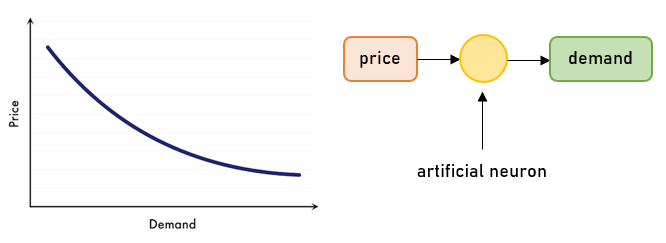
\includegraphics{deep_learning1.png}\end{center}
All this single-neuron network does is compute the curve shown and `learn' it in order to map any value of price to the appropriate value of demand. A single neuron can be thought of as a Lego brick, and a neural network as a very complicated stack, often in multiple layers, of such bricks.
\vspace{6pt}

Let's look at a more complicated example. Suppose that instead of just the price, we have more variables like shipping cost, marketing cost and material. Then we will have multiple factors that influence demand like affordability, consumer awareness and perceived quality. We might then have a slightly more complicated neural net like the one below:
\begin{center}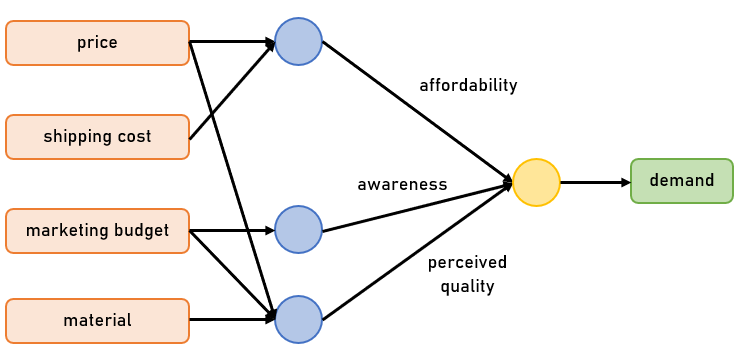
\includegraphics{deep_learning2.png}\end{center}
This slightly more complicated neural network maps the 4 input parameters to the output that is the demand.
\vspace{6pt}

From that the way in which we have discussed neural networks above, it appears as if we have to actually figure out the key factors as affordability, awareness and perceived quality. However, things do not work this way. One of the best things about neural networks is that we only have to provide it the input and the output $-$ all of the stuff in the middle, it figures out by itself. It automatically `learns' and completely trains itself to find the most accurate possible function that maps from the input to the output.
\vspace{6pt}

With this slightly advanced definition of neural networks, let us try to understand an actual practical application of neural networks in face recognition. 
\begin{center}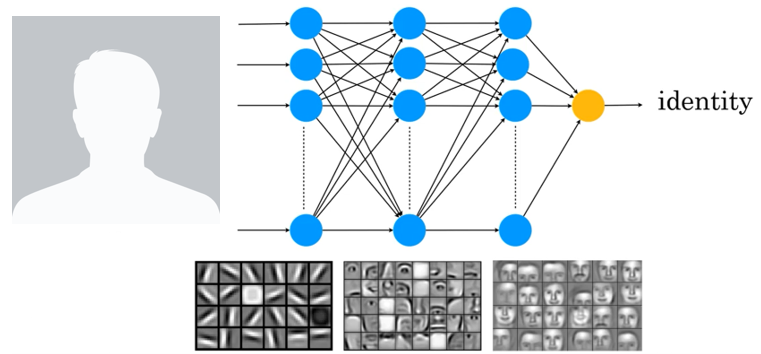
\includegraphics{face_recognition.png}\end{center}
When we look at a face, we see certain features like eyes, expression, etc. What a neural network sees is millions of RGB values for each and every pixel in the image. Typically, when you give it an image, the neurons in the earlier parts of the network will learn to detect edges in pictures and later learn to detect parts of objects. After they learn to detect eyes and noses and the shape of cheeks and the shape of mouths, the neurons in later parts of the network will learn to detect different shapes of faces and finally, will put all this together to output the identity of the person in the image.

\hrulefill
\begin{center}\textbf{END OF WEEK 1}\end{center}
This is the end of the course notes from Week 1. Keep on reading further for notes from further weeks, or spend some time gaining further insight into the previously discussed topics.

\hrulefill
\section{Building AI Projects}
So far we have covered the basics of AI and machine learning. But how do we put this technology to use in a project? Let's take a look.
\subsection{Workflow of a machine learning project}
There are 3 basic steps when building a machine learning project. Let us take speech recognition as an example, particularly Google speech recognition. How do you build a system that recognizes the words `Ok Google'?
\begin{enumerate}
	\item Collect data: involves collecting some audio clips of people saying the words `Google' and `Ok' (and lots of other words too - we want speech beyond `Ok Google' to be recognized too)
	\item Train the model: use a ML algorithm to learn input to output mappings
	\begin{itemize}
		\item[$-$] often the first attempt doesn't work very well
		\item[$-$] need to keep on iterating over the algorithm until it is good enough
	\end{itemize}
	\item Deploy the model: package the software into a product and ship it
	\begin{itemize}
		\item[$-$] may not work as well initially due to lot of new data (eg: if the sample dataset was from American users, the AI may not be able to recognize `Ok Google' from Indian users as well initially)
		\item[$-$] get back user data (while maintaining privacy regulations) to maintain and update the model
	\end{itemize}
\end{enumerate}
Let us revisit this process in another example of self-driving cars:
\begin{enumerate}
	\item Collect data: sample images and, for each of the images, position of nearby cars
	\item Train the model: invariably the first model won't work well (eg: may detect trees or rocks as cars initially); need to reiterate until the model is good enough according to safety standards
	\item Deploy the model: must be done in ways that preserve safety; get new data back (eg: new types of vehicles like tow trucks, auto rickshaws, etc) and update the model continually to the point that it can be released to the commercial market
\end{enumerate}
\subsection{Workflow of a data science project}
Unlike a ML project, the output of a data science project is a set of insights that can be used to influence business decisions. Naturally it follows that they have a different workflow compared to ML projects. Let us take the example of an e-commerce platform that sells coffee mugs. There might be several steps a user has to perform to buy the product.
\begin{center}

\includegraphics[width=\textwidth]{ecommerce_steps.png}
\end{center}
As a salesperson, it is our job to make sure that the majority of users get through all these steps. This analysis is done in a series of steps:
\begin{enumerate}
	\item Collect data: gather user info (country, time, product they checked out, price they were offered, where they quit in the buy process)
	\item Analyse data: get a data science team to work on the dataset
	\begin{itemize}
		\item[$-$] initially, the team might have a lot of ideas as to why users are not motivated to buy the product
		\item[$-$] need to iterate the analysis to get good insights and find out the major causes (eg: shipping costs are too high, so users quit at the checkout page)
	\end{itemize}
	\item Suggest hypothesis \& actions: data science team presents the insights and suggests any suitable actions (eg: incorporate part of shipping costs into product cost)
	\begin{itemize}
		\item[$-$] deploy changes to the product design and get new user data back (eg: users overseas may now buy more, but locals may not due to rise in base price)
		\item[$-$] re-analyse new data continuously to possibly come up with even better hypothesis/suggestions
	\end{itemize}
\end{enumerate}
Again, let us briefly discuss this framework in another context of optimizing a manufacturing line for coffee mugs. We will want to make sure that as little defective mugs are produced as possible:
\begin{center}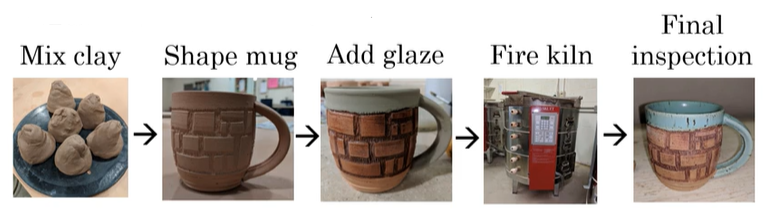
\includegraphics[scale=0.9]{manufacturing_steps.png}\end{center}
\begin{enumerate}
	\item Collect data: data about different types of clay (suppliers, mixing times, moisture content, etc) and regarding different batches of mugs (temperature of kiln, duration in kiln, defects per batch, etc)
 	\item Analyse data: ask the data science team to analyse data to find the major source of defects (eg: too high temperature might lead to softening of clay and cause mugs to crack)
	\item Suggest hypothesis \& actions: change operations (eg: vary humidity and temperature based on time of day), get dynamic feedback from manufacturing output and take further actions if necessary
\end{enumerate}
\subsection{Impact of data on job functions}
The digitization of society means that more and more data is being stored in digital formats. Due to this, almost all jobs have been or will be impacted by the advent of machine learning and data science. Let us see briefly how data science \& ML have made or are making their way into different industries:
\begin{center}
\begin{tabular}{|p{10em}|p{17em}|p{17em}|}
\hline
 & \textbf{Data Science} & \textbf{Machine Learning} \\
\hline
\textsc{Sales} & optimising a sales tunnel (refer Section 3.2) & automated lead sorting - prioritize certain marketing leads over others (contact CEO of large company over an intern at small company)\\
\hline
\textsc{Manufacturing} & optimising a manufacturing line (refer Section 3.2) & visual product inspection (AI algorithms can learn to figure out if products are defective or not)\\
\hline
\textsc{Recruiting} & optimising the recruiting process (analysing why people are not making it to certain stages or why too many people are making it) & automated resume screening based on sample dataset of resumes and whether to select candidate or not (fair and ethical screening free of any bias)\\
\hline
\textsc{Marketing} & A/B testing - launching 2 versions of a website to find out what appeals to consumers & customized product recommendations to significantly increase sales\\
\hline
\textsc{Agriculture} & crop analytics (find out what to plant and when to plant based on market conditions, soil \& weather conditions, etc) & precision agriculture (recognize presence of weeds through images/video and spray an appropriate amount of weed killers)\\
\hline
\end{tabular}
\end{center}
Of course, this list is not exhaustive and there are many more industries which have seen or will see the impact of AI soon enough.
\subsection{Choosing an AI project}
There are definitely a lot of things we can try to do with AI, but how to we choose an AI project? Let us discuss a general framework on how to choose an AI project. Many of these points have already been discussed, but let us revisit them in this context:
\begin{itemize}
	\item feasibility and value addition:
	\begin{itemize}
		\item must be feasible to do with AI and also add value to the business/application
		\item brainstorming with cross-functional teams (comprising both AI experts as well as business domain experts) to narrow down projects
	\end{itemize}
	\item brainstorming framework:
	\begin{itemize}
		\item think about automating tasks rather than entire jobs (eg: for radiologists, AI might be useful in X-ray diagnosis but not as useful in consulting with other doctors or patients)
		\item consider main drivers in business value and try to augment them using AI to increase the scale and productivity of the business
		\item consider tasks which are particularly painstaking for humans and try to automate them if possible
	\end{itemize}
	\item do not insist on acquisition of big data
	\begin{itemize}
		\item try to make progress with small datasets and get dynamic feedback from the AI team as to what type of data to obtain further and what type of IT infrastructure to build
	\end{itemize}
\end{itemize}
After brainstorming and narrowing down to a certain list of projects, it is time to pick one to work with. Committing to an AI project requires a lot of work to see it through and hence, it is important to conduct due diligence on it. Technical diligence is used to make sure the task is feasible to carry out using AI, while business diligence revolves more around deciding how much value it is going to add and if it is worth the effort.
\begin{center}
\begin{tabular}{|p{21.5em}|p{21.5em}|}
\hline
\textsc{Technical Diligence} & \textsc{Business Diligence}\\
\hline
can an AI system meet the desired performance & will automation lower costs enough?\\
\hline
how much data is needed & how much revenue/efficiency it will increase\\
\hline
engineering timeline (how long and how many people it will take) & will launching this project bring enough value to the business?\\
\hline
 & building spreadsheet financial models to estimate the value quantitatively\\
\hline
\end{tabular}
\end{center}
Another type of diligence one should try to perform is ethical diligence (i.e. is the society/environment being harmed). Any AI project should ideally add value to society and if not, it should not cause harm at least.
\vspace{6pt}

Another factor we need to consider is whether we want to build or buy (or maybe do a combination of both):
\begin{itemize}
	\item outsourcing ML projects can lead to easier access to datasets
	\item data science projects are more commonly done in-house since they are highly tied to the business (it takes very deep insider knowledge about the business which is unlikely to occur through outsourcing)
	\item try and build things that will be specialized to the project
	\item avoid building things that are an industry standard (eg: storage servers, computer hardware, etc)
\end{itemize}
\subsection{Working with an AI team}
After a project is finalised, one must know how to work with an AI team in order to make sure that the project runs smoothly. Normally a business should have already an AI team but even if not, it is fairly easy to either hire AI engineers or learn a thing or two about AI yourself and get enough knowledge to get started. After this, we need to consider the following points while working with an AI team:
\begin{itemize}
	\item specify the acceptance criteria (eg: goal is to detect defects in coffee mugs with 95\% accuracy) and provide the dataset to the AI team to measure the accuracy
	\begin{itemize}
		\item training set $-$ dataset containing both input and output using which the AI learns the mapping
		\item test set $-$ dataset with new input data which the AI team gives the algorithm to see what it outputs 
	\end{itemize}
	\item do not expect 100\% accuracy $-$ AI has its limitations and so does the amount of data being fed into the training set
	\item keep taking feedback from the AI team as to whether the training data needs to be improved, etc
\end{itemize}
It is often a good idea to be in constant touch with the AI team to try and find a reasonable level of accuracy that passes technical as well as business diligence (since it might not be worth it if the AI has low accuracy).
\pagebreak
\subsection{Technical tools for AI teams}
Let us finally discuss some of the most commonly used tools by AI teams to train and test learning algorithms. It is important to have a little knowledge about this since it gives us a better insight when communicating with the AI team.
\begin{itemize}
	\item machine learning framework: open source frameworks like PyTorch, TensorFlow, etc make writing software for ML systems much more efficient
	\item research publications: AI technology breakthroughs published freely on the internet (a major source is Arxiv) and on GitHub repositories
	\item CPUs and GPUs: CPU does majority of the computational work, while GPU hardware is very powerful for building large neural networks
	\item cloud deployments: refers to renting computer servers such as from AWS, Azure, etc to use external servers to do the computation (as opposed to on-premises deployment, which means buying your own servers)
	\item edge deployment: putting a processor right where data is collected to process data and make quick decisions
	\begin{itemize}
		\item for a self-driving car, there is not enough time to record data, send data to a cloud server and receive a response from the server
		\item computation must happen quickly inside the car
	\end{itemize}
\end{itemize}
\hrulefill
\begin{center}
\textbf{END OF WEEK 2}
\end{center}
This is the end of the course notes from Week 2. Keep on reading further for notes from further weeks, or spend some time gaining further insight into the previously discussed topics.

\hrulefill
\pagebreak
\section{Building AI in a Company}
Up till now, we have discussed what AI is and how to build an AI project. Let us now discuss some complex AI projects in depth and find out how AI projects fit in the context of a company.
\subsection{Smart speakers: a case study}
Let us go through a brief case study of how AI software is written to respond to voice commands like `Ok Google, tell me a joke'. There is a sequence of steps (known as an AI pipeline) needed to process the command:
\begin{center}
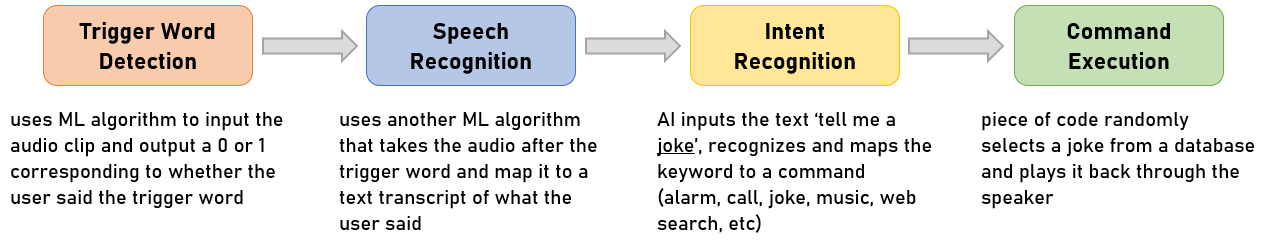
\includegraphics[width=\textwidth]{smart_speaker_steps1.png}
\end{center}
Quite often, AI teams are split into various specialized groups and each of them focus on specific tasks in the AI pipeline. The AI pipeline is reasonably flexible in that it might change on occurrence of a slightly more complicated command like `Ok Google, set a timer for 3 minutes'.
\vspace{6pt}

In such a case, majority of the earlier process remains the same except the final step. The execution step will be separated into 2 further steps:
\begin{itemize}
	\item extract duration $-$ look at the text and pull out the phrase corresponding to the time duration
	\item command execution $-$ specialized software component that can start a timer with the set duration
\end{itemize}
Smart speakers have a lot more functions apart from the above two and given the function we want to perform, we can figure out what the AI pipeline will look like. A major challenge for teams building a smart speaker lies in the intent recognition stage - a user can ask for a particular command in many ways (eg: tell me a joke, do you know any good jokes?, say something funny, make me laugh, etc).
\vspace{6pt}

To further solidify our understanding of the AI pipeline, let us look at a second case study on self-driving cars.
\subsection{Self-driving cars: a case study}
Let us try to construct the AI pipeline of how the AI in a self-driving car might make decisions on how to drive.
\begin{center}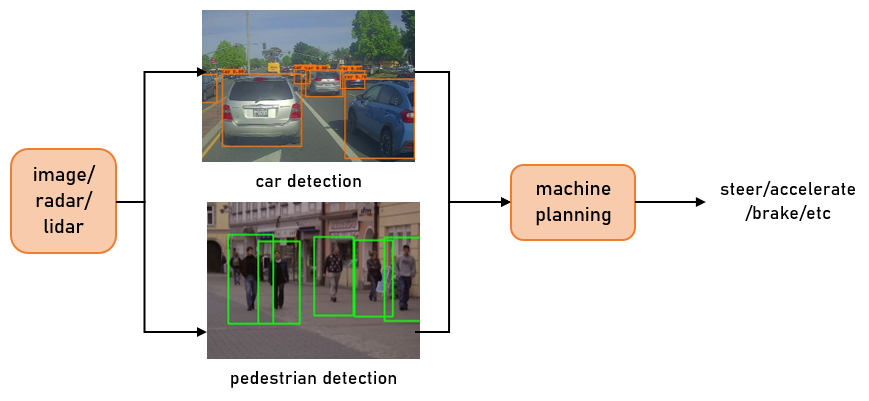
\includegraphics[scale=0.8]{self_driving_car_steps.png}\end{center}
Let us look into some details regarding car detection, pedestrian detection and motion planning:
\begin{itemize}
	\item car detection $-$ supervised learning algorithm to input images from all sides of the car, radar info and output positions of nearby cars
	\item pedestrian detection $-$ very similar to car detection techniques
	\item motion planning $-$ outputs the path the car should take as well as safe speed to avoid collisions with other cars (as well as overtaking parked cars)
\end{itemize}
This is a fairly simplified pipeline of how a self-driving car might work. Most self-driving cars would have an auto navigator that relies on GPS, and also use other stuff like gyroscopes. 
\vspace{6pt}

Another component in self-driving cars is that of trajectory prediction. Instead of just knowing the current position of cars, it is more useful to be able to predict how they are likely to move in the next few seconds (by focusing on turn indicators, brake lights, etc) to be able to avoid them even as they are moving. To drive safely we need to consider a lot of other factors, which might lead to a fairly complicated AI pipeline as below:
\begin{center}
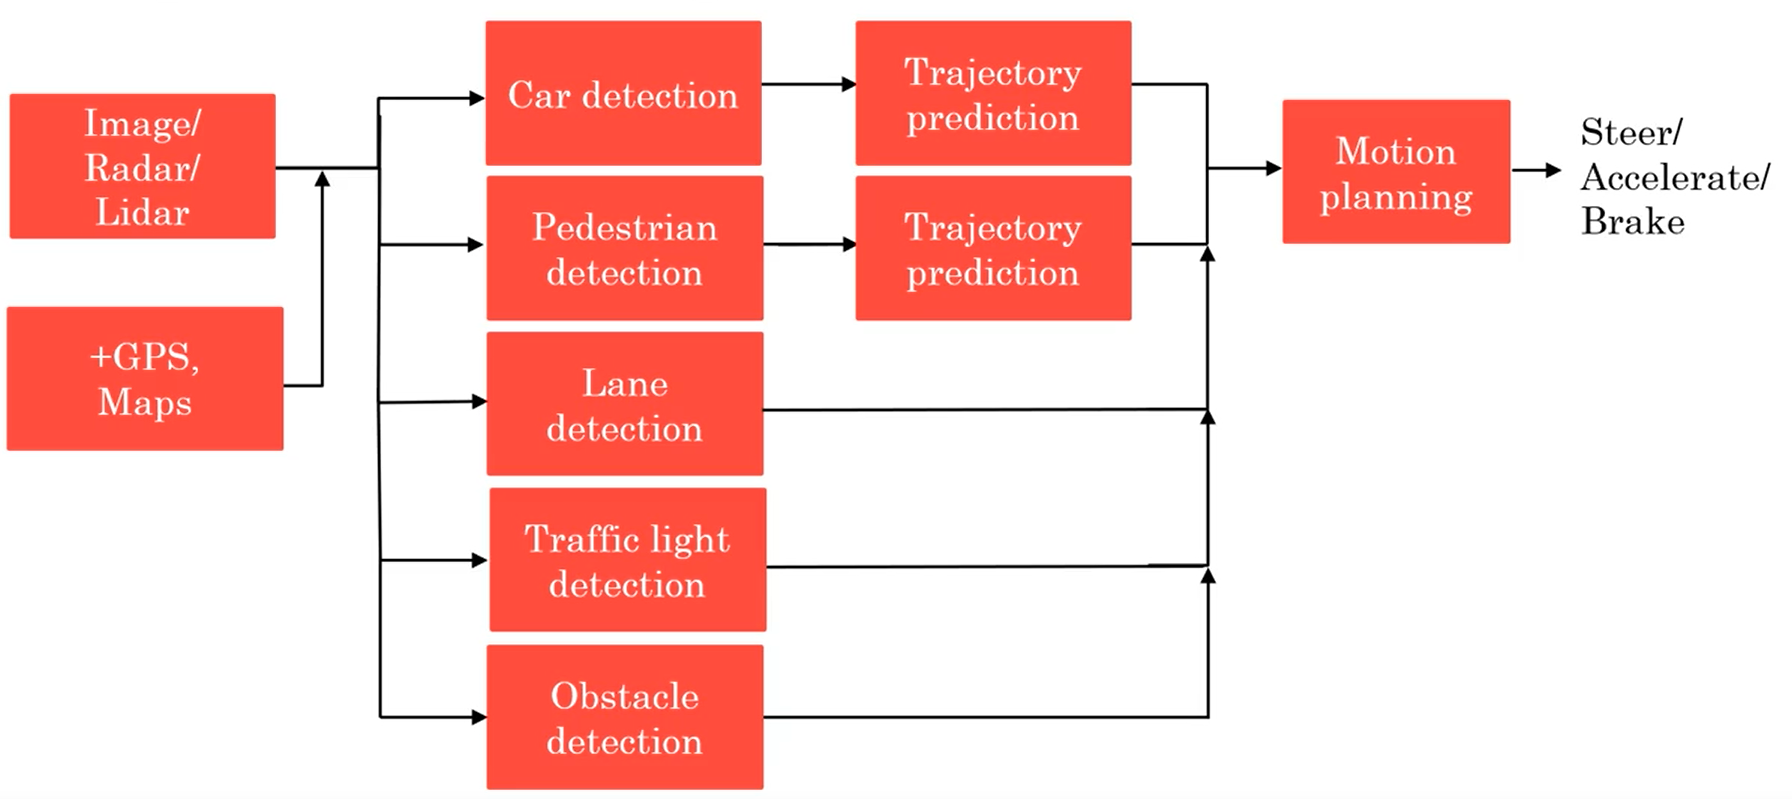
\includegraphics[width=\textwidth]{self_driving_pipeline.png}
\end{center}
\subsection{Major roles in an AI team}
In the previous example of a self-driving car, we saw a pretty complicated AI pipeline. To pull off a project like this, there are usually large AI teams divided into small groups to work on specialized tasks. Let's take a look into the major roles in such a team:
\begin{itemize}
	\item software engineer: write specialized software for command execution
	\item machine learning engineer: write software responsible for A $\rightarrow$ B mappings, collect data and train neural networks by interating over the algorithm
	\item machine learning researcher: perform research on how to extend state-of-the-art in ML, publish papers and maintain documentation
	\item machine learning scientist: go through academic \& research literature to find ways to implement state-of-the-art technology to the current application
	\item data scientist: examine data and gain insights; further discuss and present the insights to the team
	\item data engineer: organize data and saving it in an easily accessible, secure and cost-effective way
	\item AI product manager: help decide what is feasible and valuable, and what to finally build; manage deadlines and coordinating with the team
\end{itemize}
Even though having a large team generally helps due to the possibility of specialized jobs, it is possible to get started with a relatively small team of about 3-5 people. Even a basic knowledge can help to start analysing small amounts of data and training basic ML models.
\vspace{6pt}

Up till now, we have seen what an AI team comprises, but AI teams often need to work with other departments in the company to bring out maximum efficiency. This is where the AI transformation playbook comes in.
\subsection{The AI transformation playbook}
Just having a large AI team at its disposal does not make a company a good AI company. Many of the top AI companies follow most of the points in the AI transformation playbook in some way of the other (this is a term coined by Andrew Ng, a pioneer in ML technology who also happens to be the instructor for this course, but is essentially a list of points that, if followed, is likely to make a company good at AI):
\begin{enumerate}
	\item Execute pilot projects to gain momentum
	\begin{itemize}
		\item initial project should be successful rather than valuable (helps gain the confidence of other departments in the company and investors)
		\item project should preferably show quick traction (within 6-12 months) since it helps gain the required momentum and experience for future projects
		\item can outsource data initially to work upon it and gain experience before building an in-house team
	\end{itemize}
	\item Build an in-house AI team
	\begin{itemize}
		\item centralized AI team instead of each business unit having their own AI component
		\item build company-wide platforms (software tools, data infrastructure, etc)
	\end{itemize}
	\item Provide broad AI training
	\begin{itemize}
		\item executives and seniors should know the basics of AI and how to make resource allocation decisions
		\item AI division leaders should know how to conduct diligence on projects before selecting them and monitor the progress of different teams working on the project
		\item AI engineers/trainees should be able to collect the right type of data, build algorithms based off of it and then assemble various modules of the project to ship it 
	\end{itemize}
	\item Develop an AI strategy
	\begin{itemize}
		\item leverage AI to create an advantage specific to the industry sector
		\item this point is not at number one because before planning out a strategy, it is important to have basic knowledge regarding AI (for example, one may put forth a strategy to collect a lot of data, but is that data really useful?)
		\item the virtuous cycle of AI:
		\begin{itemize}
			\item better product $\rightarrow$ more users $\rightarrow$ more user data (which can be used to update the model) $\rightarrow$ better product (and so on)
			\item difficult for newer companies to enter the market since already existing companies are likelier to have a better product and larger user base
			\item small teams can take advantage of this by pushing into lesser explored industries and capitalizing later on their specialization
		\end{itemize}
		\item strategic data acquisition (eg: launching free services solely for data collection purposes)
		\item unified data warehouses let engineers connect the dots (eg: in case of customer complaints, it is better to have the manufacturing data in the same place to find out exactly what caused the fault)
	\end{itemize}
	\item Develop internal and external communications
	\begin{itemize}
		\item how AI will benefit the company must be communicated to investors so relations are maintained
		\item communicate with the government to introduce AI solutions in areas like health care, and even other areas where user privacy regulations are strict
		\item user education as to how to deal with introduction of new technology
		\item may also help in recruitment procedures for the company
	\end{itemize}
\end{enumerate}
If you wish to go through the entire AI transformation playbook in much greater detail, you may do so here: \texttt{\href{https://landing.ai/ai-transformation-playbook/}{https://landing.ai/ai-transformation-playbook/}}.
\subsection{First steps and pitfalls}
Even after following all the points in the AI transformation playbook, there are companies which are subject to common pitfalls while taking their first steps towards an AI project.  Let us look at some of them:
\begin{itemize}
	\item expecting AI to solve everything (instead, one should give due time to technical and business diligence to figure out if the project is actually possible and valuable using AI)
	\item hiring employees of only one type i.e. only ML engineers or only software engineers, etc (there should be a cross-functional team that pairs business talent with engineering talent)
	\item expecting AI projects to work right away (more often the first attempt is a disaster, but continuous iteration of training data over the algorithm can refine it a lot)
	\item expecting traditional business approaches to work (instead, one should build a separate AI team and work with them for a more dynamic progress)
	\item feeling the need to have a large team and a huge amount of data (often small teams working with small datasets can gain better insights before investing further in data collection)
\end{itemize}
Much of what we have discussed so far might sound great but can feel daunting when it comes to putting things to practice. In order to take the first step into the world of AI, it is better to get a certain group (maybe a group of friends) to learn about AI instead of going in solo. It is also important to brainstorm on different projects, even if they seem to small - it is better to start small and succeed rather than to go big and fail.
\vspace{6pt}

Now that we have looked through the basics of AI technology and how to build and choose AI projects, let us now go through slightly more advanced concepts like reinforcement learning, computer vision, natural language processing, etc.
\subsection{Major AI application areas}
AI today is being successfully applied in many industries involving image \& video data, language data, speech data, etc. Let's take a deeper look into a brief survey of of how AI is applied to these different areas.
\subsubsection{Computer vision}
One of the major successes of deep learning has been computer vision. To understand what computer vision is, let us look at some of its applications.
\vspace{6pt}

One of these applications is image classification/object recognition. For example, AI can take a picture and tell the user if it is of a cat. This technology is actually much more advanced than just recognizing cats $-$ there are applications to detect certain species of flowers, types of food, etc. And of course, one of the major implementations of this lies in face recognition.
\vspace{6pt}

Another type of computer vision algorithm is that of object detection. Hence rather than just recognize an object and label the whole image, we're trying to detect the different types of objects in the same image. For example, a self-driving car AI does not only recognize cars \& pedestrians but also shows their position. It is also possible to track the live position of cars, etc as they are moving.
\vspace{6pt}

Image segmentation takes this one step further $-$ it tells us not just where the cars are but also for every single pixel in the image, if that pixel is a part of a car or of a pedestrian, etc. This is commonly used in X-ray scans to detect particular organs.
\subsubsection{Natural language processing}
NLP refers to AI understanding everyday human language. One application of NLP lies in text classification (eg: to take an email and categorize it as spam or not spam, or take a product description and figure out which category it belongs to).
\vspace{6pt}

One type of text classification used widely is sentiment recognition \& analysis. This type of AI can take input like ``The food was good, but the ambience can be improved'' and output an expectation of the star rating the restaurant might get.
\vspace{6pt}

A second type of NLP is information retrieval, of which web search is probably the best example. This AI will take in a search string as input and help the user find relevant documents. Companies also use this internally to search within particular sets of documentation.
\vspace{6pt}

Name entity recognition is another type of NLP, which helps filter out certain types of names in large documents. For example, the input `I am fluent in English, Spanish and Japanese' should lead the NLP algorithm to filter out English, Spanish and Japanese as language names. They can also recognize phone numbers, countries, etc.
\vspace{-6pt}

NLP also features in applications of machine translation, where the AI translates an input phrase or document into a specific language that the user wants. Apart from the above, NLP can be used in a wide range of other applications like parsing, part-of-speech tagging (classify which words in a string are nouns, verbs, etc), etc. 
\subsubsection{Speech}
Modern AI technology has completely transformed how speech is processed by computers. A microphone records rapid variations in surrounding air pressure. These variations can be represented on a plot against time on a computer (this is the information a typical digital audio waveform contains). Speech recognition deals with taking inputs of a plot like this and figure out what the user said.
\vspace{6pt}

As we discussed earlier, one particular type of speech recognition is trigger word/wakeword detection. Another type of speech recognition used is speaker ID, where the problem is to take an audio clip and figure out the identity of the speaker.
\vspace{6pt}

Recently, text-to-speech has also gained a lot of traction. TTS is used in audio books and as aid in communication for people lacking the ability of speech.
\subsubsection{Robotics}
One of the applications in robotics we have already seen is that of a self-driving car. One of the main challenges with robotics are perception (figuring out what is in the world around us), motion planning (computing a path for the robot to follow) and control (sending commands to motors \& other electric components to execute the calculated path).
\subsubsection{General machine learning}
A majority of the applications we saw dealt with unstructured data. However ML works just as well for structured data. Structured data processing is often more specific to a company and it is harder for humans to understand the data at first glance and/or empathize with it.
\subsection{Major AI techniques}
In the previous sections, we have mainly discussed only supervised learning. This term almost invites the question as to what is unsupervised learning? Apart from this, there are other AI techniques like reinforcement learning as well.
\subsubsection{Unsupervised learning}
The best known example of unsupervised learning is that of clustering. Suppose there is a shop that specializes in selling chocolates. It may sell cheap, low quality chocolates as well as expensive but high quality ones. If consumer buying patterns are plotted on a graph, it may reveal that buyers are separated into 2 groups $-$ some buy a lot of cheap chocolates while others buy a few expensive chocolates. A clustering algorithm automatically sorts this data into 2 clusters and this data can be used for market segmentation (for example, in an area with a nearby university, college students are more likely to buy cheaper chocolates so it would make more sense for the shop to stock the cheap ones). 
\vspace{6pt}

Unlike supervised learning, an unsupervised learning algorithm does not tell a system exactly what output  it wants. Instead what it does is feed the data and ask the system to find something peculiar or meaningful. In the above example, the algorithm just finds what are the different market segments without being told they belong to college students or working people, etc.
\vspace{6pt}

Unsupervised learning overcomes one of the major criticisms against supervised learning, which is that it requires a lot of labelled data. This opens a possibility to AI being able to learn much more like a human from much lesser data in the future.
\subsubsection{Transfer learning}
Say we have built an algorithm for self-driving cars and start deploying it. There might be regions with different types of vehicles like golf carts. Even though our system has been trained with a lot of data, it will contain very few images of golf carts. Instead of building another algorithm for golf cart detection from the ground up, we can use the technique of transfer learning. This technique lets us learn from task A and use the knowledge to help with task B. It particularly works very well if the dataset from task A is large.
\subsubsection{Reinforcement learning}
Let's say we want to write an algorithm for automating a helicopter. It is difficult to do this by supervised learning because, while in the case of card we had only a few types of objects to deal with, here we have a lot more. It is very difficult to specify what is the best way to fly an helicopter when it is in a certain position. This is where reinforcement learning comes in.
\vspace{6pt}

It is quite similar to how one would train a pet. A simulation is created to let the helicopter fly around. Whenever the AI flies the helicopter well, we give it a positive feedback and when it crashes, we give it a negative feedback. Over time, the AI learns how to fly the helicopter as it keeps on getting dynamic feedback. More formally, reinforcement learning uses a `reward signal' to tell the AI whether it is doing well or poorly $-$ it automatically learns to maximize its positive rewards.
\vspace{6pt}

In addition to this, reinforcement learning has also helped build algorithms for playing strategic games like Othello or chess, and also for playing video games. One of the weaknesses of reinforcement learning is that it is difficult to control the amount of data the system feeds to its own learning algorithm.
\subsubsection{GANs (generative adversarial networks)}
This AI technique was only recently designed in 2014. GANs are very good at synthesizing images from scratch. This aspect has caused GANs to gain a lot of traction in everything involved with computer graphics like video games and other media.
\vspace{6pt}

The general idea of GANs is of 2 networks (generative and discriminative) working hand in hand. The generative network generates stuff while the discriminative network evaluates it. The job of the generative network is to increase the error rate of the discriminative network (i.e. to try and fool the discriminative network as much as possible by producing novel images based on a true data distribution that the discriminative network thinks are not actually synthesized).
\subsubsection{Knowledge graph}
One of the more underrated AI techniques are knowledge graphs. A web search about a famous personality often leads in a huge string of links and a panel to the right showing some of their general details. These details are derived from a knowledge graph, which is nothing but a database that lists people and key information about them. Many companies build such databases of celebrities, movies, hotels, etc and can help extract a lot of important data relatively quickly.

\hrulefill
\begin{center}
\textbf{END OF WEEK 3}
\end{center}
This is the end of the course notes from Week 3. Keep on reading further for notes from further weeks, or spend some time gaining further insight into the previously discussed topics.

\hrulefill
\pagebreak
\section{AI and Society}
We have already seen how much AI is capable of. It can affect people's lives on a mass scale, especially when huge companies implement AI solutions. While all this sounds great, is it also important to consider the social impact of an AI project and make sure that the project will not harm society/environment in any manner.
\subsection{A realistic view of AI}
Given the huge impact AI is having on society, it is important for us to have a realistic view of AI and be neither too pessimistic nor too optimistic. AI has been hyped up to the point that a lot of people believe super-intelligent AI robots will completely take over the world and that it is important to invest into defending the world against evil AI bots. It is only causing distractions and unnecessary fears.
\vspace{6pt}

On the flip side, there are people who believe that we expect too much of AI and another `AI winter' is coming (this refers to past events where people were too excited for AI but then later found it couldn't do what they wanted, and so abandoned it altogether). The difference between AI then and now is that AI today is creating a huge economic value and it is possible to clearly visualize how it will affect industries in the near future.
\vspace{6pt}

We previously discussed in detail the performance limitations of AI, but here are some more that affect how society views AI:
\begin{itemize}
	\item many high-performing AI systems are black boxes $-$ since people have not actually worked with the AI team, they have no first-hand proof of reliability of the AI system (i.e. how the AI system does what it does) and hence end up rejecting the value it can bring
	\item biased AI through biased data $-$ behaviour of the AI is dependant on the data using which it is trained (hence if fed biased data, the resulting AI will also naturally learn this bias)
	\item some AI systems might be open to adversarial attacks, i.e. if someone deliberately tries to fool the AI
\end{itemize}
\subsection{Discrimination and biases}
Many AI teams today rely on the internet for access to cheap data. It is no secret that the internet is full of biases and unhealthy stereotypes, and this really affects many AI products. For example, a recent research by Microsoft concludes the following:
\begin{center}
on asking the AI $\rightarrow$ man : woman as father : (answer), the AI answers `mother' (okay so far)

on asking the AI $\rightarrow$ man : woman as king : (answer), the AI answers `queen' (still reasonable)

on asking the AI $\rightarrow$ man : programmer as woman : (answer), the AI answers `homemaker'
\end{center}
No AI team has intentions of training a biased AI system, but such things can really hurt how AI is viewed by society. Let us take a deeper look at how AI develops such biases:
\begin{itemize}
	\item AI stores words as a set of numbers (these numbers are auto-generated by the AI based on statistics of how that word is used on the internet)
	\item `Man' may be stored as (1,1) $-$ in practice there might be thousands of numbers, but let us work with a set of 2 numbers for now
	\item let's say `Programmer' : (3,2) and `Woman' : (2,3) which, if plotted, looks like this
\end{itemize}
\begin{center}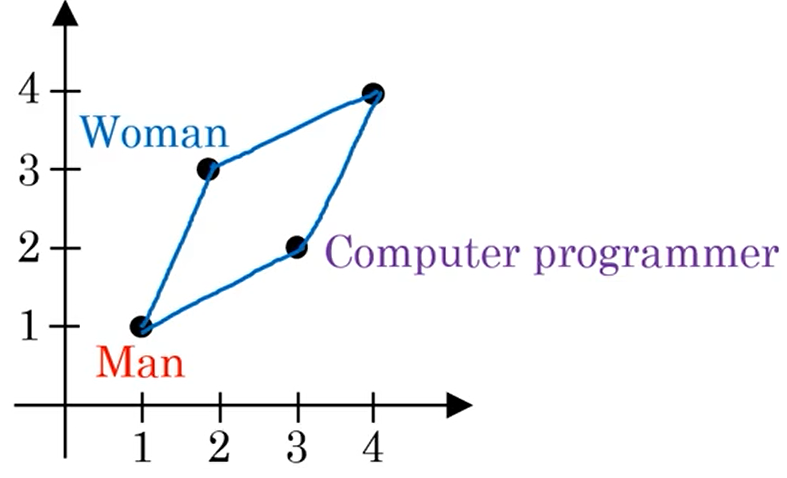
\includegraphics[scale=0.4]{word_plot.png}\end{center}
What the AI system will do to map `Woman' to an answer is construct a parallelogram as above and search for the word stored in (4,4). Based on files from the internet, this word happens to be `Homemaker'.
\vspace{6pt}

There are many situations where such a bias matters. For example, it is unfair if a resume screening AI for a job application has such biases. Other types of biases also exist:
\begin{itemize}
	\item face recognition seems to work more accurately for light-skinned people compared to those with darker skin
	\item bank loan approval systems have ended up discriminating against some ethnic minorities
	\item web search algorithms showing men in leading job positions may have a negative effect on women trying to pursue similar careers
\end{itemize}
The AI community is continuously working to make AI systems as free from bias as possible. Researchers have learned that when an AI learns a word as a set of numbers, only a few numbers out of those contribute to the bias. If we zero out these numbers, the bias can be greatly reduced. Another solution is to use less biased data or data that has reasonable sized samples from multiple ethnicities and all genders as well.
\vspace{6pt}

Secondly, many AI teams are subjecting their systems to auditing processes, where-in a third-party auditing team evaluates the fairness of the AI system and provides suggestions on what types of biases exist. This greatly increases the odds of a bias (or any other performance issue as well) being spotted so that it can be fixed.
\vspace{6pt}

Finally, it also helps if AI teams have a diverse workforce. This allows people to spot problems that might not look like problems to other people. With these implementations, the bias in AI can be greatly mitigated.
\subsection{Adversarial attacks on AI}
While AI is particularly good at reading stuff that is illegible to humans like barcodes and QR codes, it can be fooled by slight changes to data that no human would be fooled by. A major reason for this is that AI looks at data in a discrete manner (i.e. discrete numerical values). For example, even minor changes in pixel values of an image can cause an AI to classify objects as something else entirely.
\begin{center}
\includegraphics[scale=0.6]{adversarial_attacks.png}\end{center}
There might be other ways in which people can fool AI systems. For example, some people were able to design a pair of funky glasses that made a face recognition system falsely recognise a person as the actress Milla Jovovich. As another example, AI sometimes fails to recognize stop signs if there are stickers or graffiti applied over it.
\vspace{6pt}

There are various defenses against adversarial attacks, but these incur high costs (and also cause the system to possibly run slower). Neural networks can be modified dynamically to make them somewhat harder to attack. Unfortunately, this is an area where no amount of advancement is enough since attackers will constantly come up with strategies to try and fool AI systems.
\subsection{Adverse uses of AI}
While most of AI is designed to make the society better off, AI can also be used in adverse situations like those listed below:
\begin{itemize}
	\item DeepFakes $-$ synthesizing videos of people doing things they never did to target individuals/companies
	\item generating fake comments $-$ especially harmful in cases of business statements and political matters 
	\item oppressive surveillance $-$ performing surveillance even in cases where it violates laws of privacy
\end{itemize}
It is very difficult to stop use cases of AI like this. Take the first example. Even though technologies exist to identify deepfakes, fake news generally spreads much quicker than the truth due to social media platforms.
\subsection{AI and developing economies}
While big AI products are generally built in developed countries, AI is making it into developing countries and impacting them as well. In fact, many developing economies have seen success by using AI to capitalize more on their existing strengths (eg: a country may be good at agriculture, textile and so on). This allows them to shift human resources to build infrastructure in other sectors that they might possibly be weak at.
\vspace{6pt}

Because education in AI is still immature, it may also help developing economies to invest in AI education so that it can build its own AI workforce and contribute to the overall economic value created by AI in the future.
\subsection{AI and jobs}
Even before the advent of AI, automation had a large impact on jobs. Now, with AI, the set of things we can automate is suddenly a whole lot more. Due to this, many jobs are being replaced through automation while many jobs are also being simultaneously created. According to a study by McKinsey Global Institute, by 2030, AI will have displaced between 400-800 million jobs while also having created between 555-890 million jobs.
\vspace{6pt}

Of course, certain jobs are more likelier to be displaced by AI. Since AI projects usually aim at applying AI to certain tasks instead of entire jobs, it is quite less likely that highly complicated jobs will be displaced by AI in the near future. Here is a brief list of jobs sorted according to their likelihood of being displaced by AI:
\begin{center}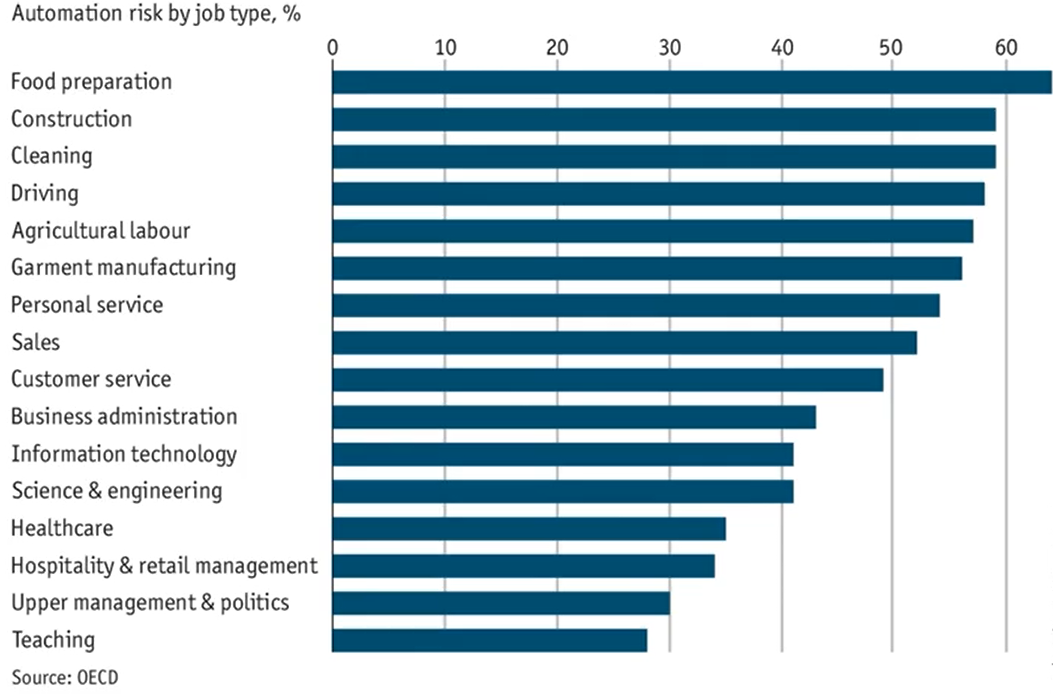
\includegraphics[scale=0.6]{automation_risk.png}\end{center}
It should not come as a surprise that many of the top jobs in the list above involve routine repetitive tasks. On the other hand, jobs involving fairly diverse tasks or social interaction are much less susceptible to automation.
\vspace{6pt}

Finally, let us discuss some solutions that can help people navigate the impact of AI on jobs:
\begin{itemize}
	\item conditional basic income $-$ governments can provide a basic income or change tax patterns to give people an incentive to learn and invest in their own development
	\item lifelong learning $-$ people should keep on learning to be in a better position to adapt and take advantage of new jobs being created
	\item political solutions $-$ incentives for new job creation (i.e. people to move into AI-related jobs)
\end{itemize}
If a person has the ability to combine their knowledge of AI with their work-related knowledge, it makes them more uniquely qualified to do very valuable and efficient work.

\hrulefill
\begin{center}
\textbf{END OF WEEK 4}
\end{center}
This is the end of the notes for this course. If you have any feedback or wish to browse through notes for other courses, you may do so using the links on my website - \texttt{\href{https://omprabhu31.github.io/}{https://omprabhu31.github.io/}}.

\hrulefill
\end{document}
